
Inicialmente se lee sobre las herramientas de diseños FIR en MATLAB \texttt{fir1}, \texttt{fir2} y \texttt{firpm}. Sobre dichos comandos se puede comentar que:
\begin{itemize}
    \item \texttt{fir1}: Diseño de filtro FIR basado en ventanas. Retorna los coeficientes $b$ de un filtro FIR en base a un orden dado, una ventana y el tipo que se requiera. 
    %b = fir1(n,Wn,ftype) designs a lowpass, highpass, bandpass, bandstop, or multiband filter, depending on the value of ftype and the number of elements of Wn.
    \item \texttt{fir2}: Diseño de filtro FIR basado en muestreo de la respuesta en frecuencia. Retorna los coeficientes $b$ de un filtro FIR en base a un orden dado y a un set de puntos de la magnitud de la respuesta en frecuencia. 
    %b = fir2(n,f,m) returns an nth-order FIR filter with frequency-magnitude characteristics specified in the vectors f and m. The function linearly interpolates the desired frequency response onto a dense grid and then uses the inverse Fourier transform and a Hamming window to obtain the filter coefficients.
    \item \texttt{firpm}: Diseño de filtro FIR óptimo dado una respuesta en frecuencia deseada usando el algoritmo Parks-McClellan. En secciones posteriores se analizará más en detalle.
    %Parks-McClellan optimal FIR filter design
    %firpm designs a linear-phase FIR filter using the Parks-McClellan algorithm [2]. The Parks-McClellan algorithm uses the Remez exchange algorithm and Chebyshev approximation theory to design filters with an optimal fit between the desired and actual frequency responses. The filters are optimal in the sense that the maximum error between the desired frequency response and the actual frequency response is minimized.
\end{itemize}

\begin{enumerate}
\item En primer lugar se diseñan filtros FIR de orden 70, frecuencia de corte 3 kHz y frecuencia de muestreo 16 kHz, usando ventana rectangular y blackman, con el comando \texttt{fir1}.

La sección de código utilizada se muestra a continuación.
\begin{lstlisting}[frame=single]
%%% 1. Diseno de filtros FIR usando fir1

%orden
n1 = 70;
%frecuencia de corte normalizada
Fs = 16000; fc_Hz = 3000; fc = fc_Hz/(Fs/2);
%ventanas
win11 = ones(n1+1,1);win12 = blackman(n1+1);
%diseno
a1 =[1 zeros(1,n1-1)];
b11 = fir1(n1,fc,win11); b12 = fir1(n1,fc,win12);
\end{lstlisting}

Los gráficos de la respuesta en frecuencia de los filtros diseñados con ventana rectangular y blackman se muestran en las figuras \ref{fig:p3_1_rect} y \ref{fig:p3_1_blackman} respectivamente. Se aprecia que:
\begin{itemize}
    \item En el caso del filtro diseñado con ventana de rectangular se observa una región de transición más corta y menos atenuación en la banda de rechazo.
    \item El filtro diseñado con ventana blackman presenta una atenuación mayor en la banda de rechazo.
    %\item La región de fase lineal es mayor en el filtro diseñado con ventana blackman. Cabe destacar que en temas prácticos esta ventaja debiese ser poco notoria ya que la región de fase no lineal se encuentra en la banda de rechazo y por lo tanto es poco probable que se aprecie una distorsión significativa en la forma de onda.
\end{itemize}

\begin{figure}[H]
    \centering
    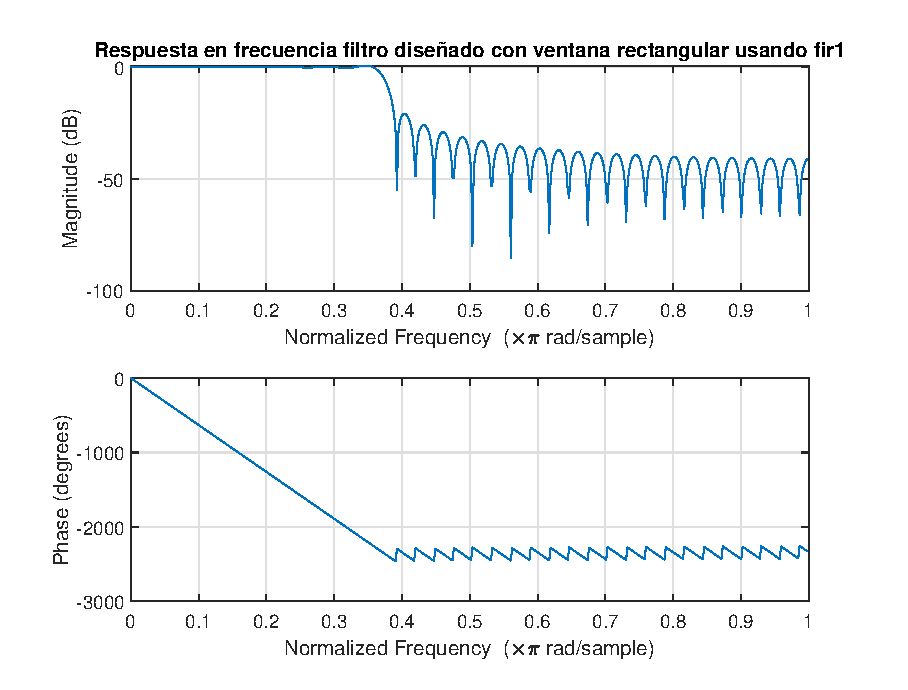
\includegraphics[width = .8 \linewidth]{Figuras/p1_31_rect.eps}
    \caption{Respuesta en frecuencia filtro diseñado con ventana rectangular usando \texttt{fir1}.}
    \label{fig:p3_1_rect}
\end{figure}
\begin{figure}[H]
    \centering
    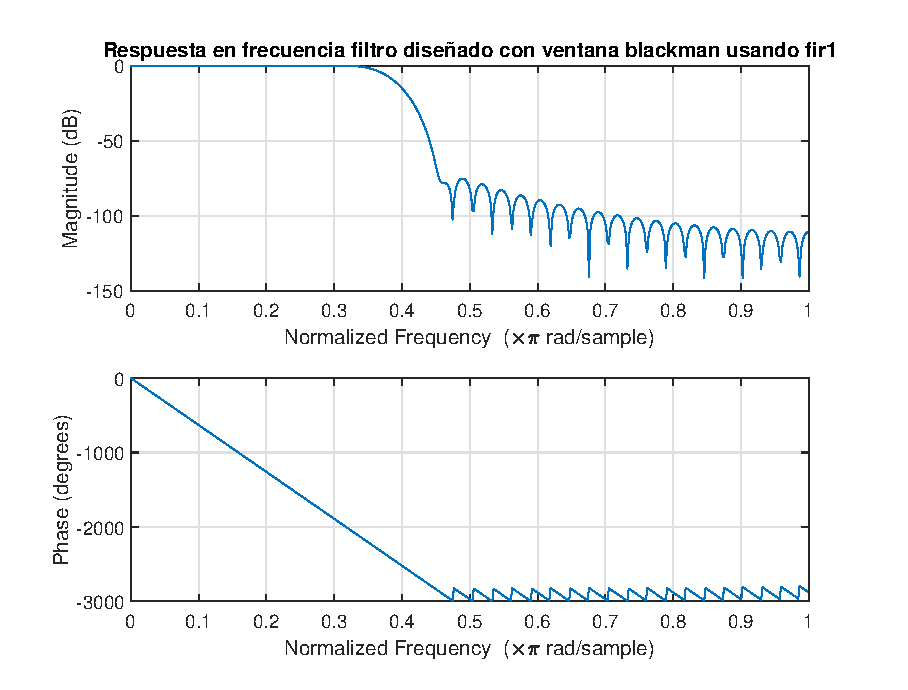
\includegraphics[width = .8 \linewidth]{Figuras/p1_31_blackman.eps}
    \caption{Respuesta en frecuencia filtro diseñado con ventana blackman usando \texttt{fir1}.}
    \label{fig:p3_1_blackman}
\end{figure}

\item Se pide encontrar el filtros de orden 70 y 150 usando el comando \texttt{fir2} de MATLAB, el cual recibe el orden del filtro y un set de puntos de respuesta en frecuencia los cuales son interpolados linealmente. La respuesta en frecuencia ideal a emular se muestra en la figura \ref{fig:p3_2_obj}
\begin{figure}[H]
    \centering
    \includegraphics[width = .8 \linewidth]{Figuras/p3_2_obj.png}
    \caption{Respuesta en frecuencia ideal a emular.}
    \label{fig:p3_2_obj}
\end{figure}

La sección de código con la cual se diseñan los filtros se muestra a cotinuación:
\begin{lstlisting}[frame = single]
%%% 2. Diseno de filtros FIR usando fir2

%orden 
n21 = 70; n22 = 150;
%Objetivo en frecuencia
f_obj = [0 .1 .15 .35 .4 .65 .75 1];
h_obj = [1  1   0   0 .5  .5   0 0];
%diseno
b21 = fir2(n21,f_obj, h_obj); b22 = fir2(n22,f_obj, h_obj);
\end{lstlisting}
donde simplemente se reconocieron los puntos en la respuesta en frecuencia tal que al interpolar linealmente se llegara a la respuesta en frecuencia ideal.

En primer lugar se grafica la magnitud de la respuesta en frecuencia del filtro ideal y los 2 diseñados, lo cual se muestra en la figura \ref{fig:p3_2_fr1}. Se aprecia un diseño correcto según las especificaciones en frecuencia.
\begin{figure}[H]
    \centering
    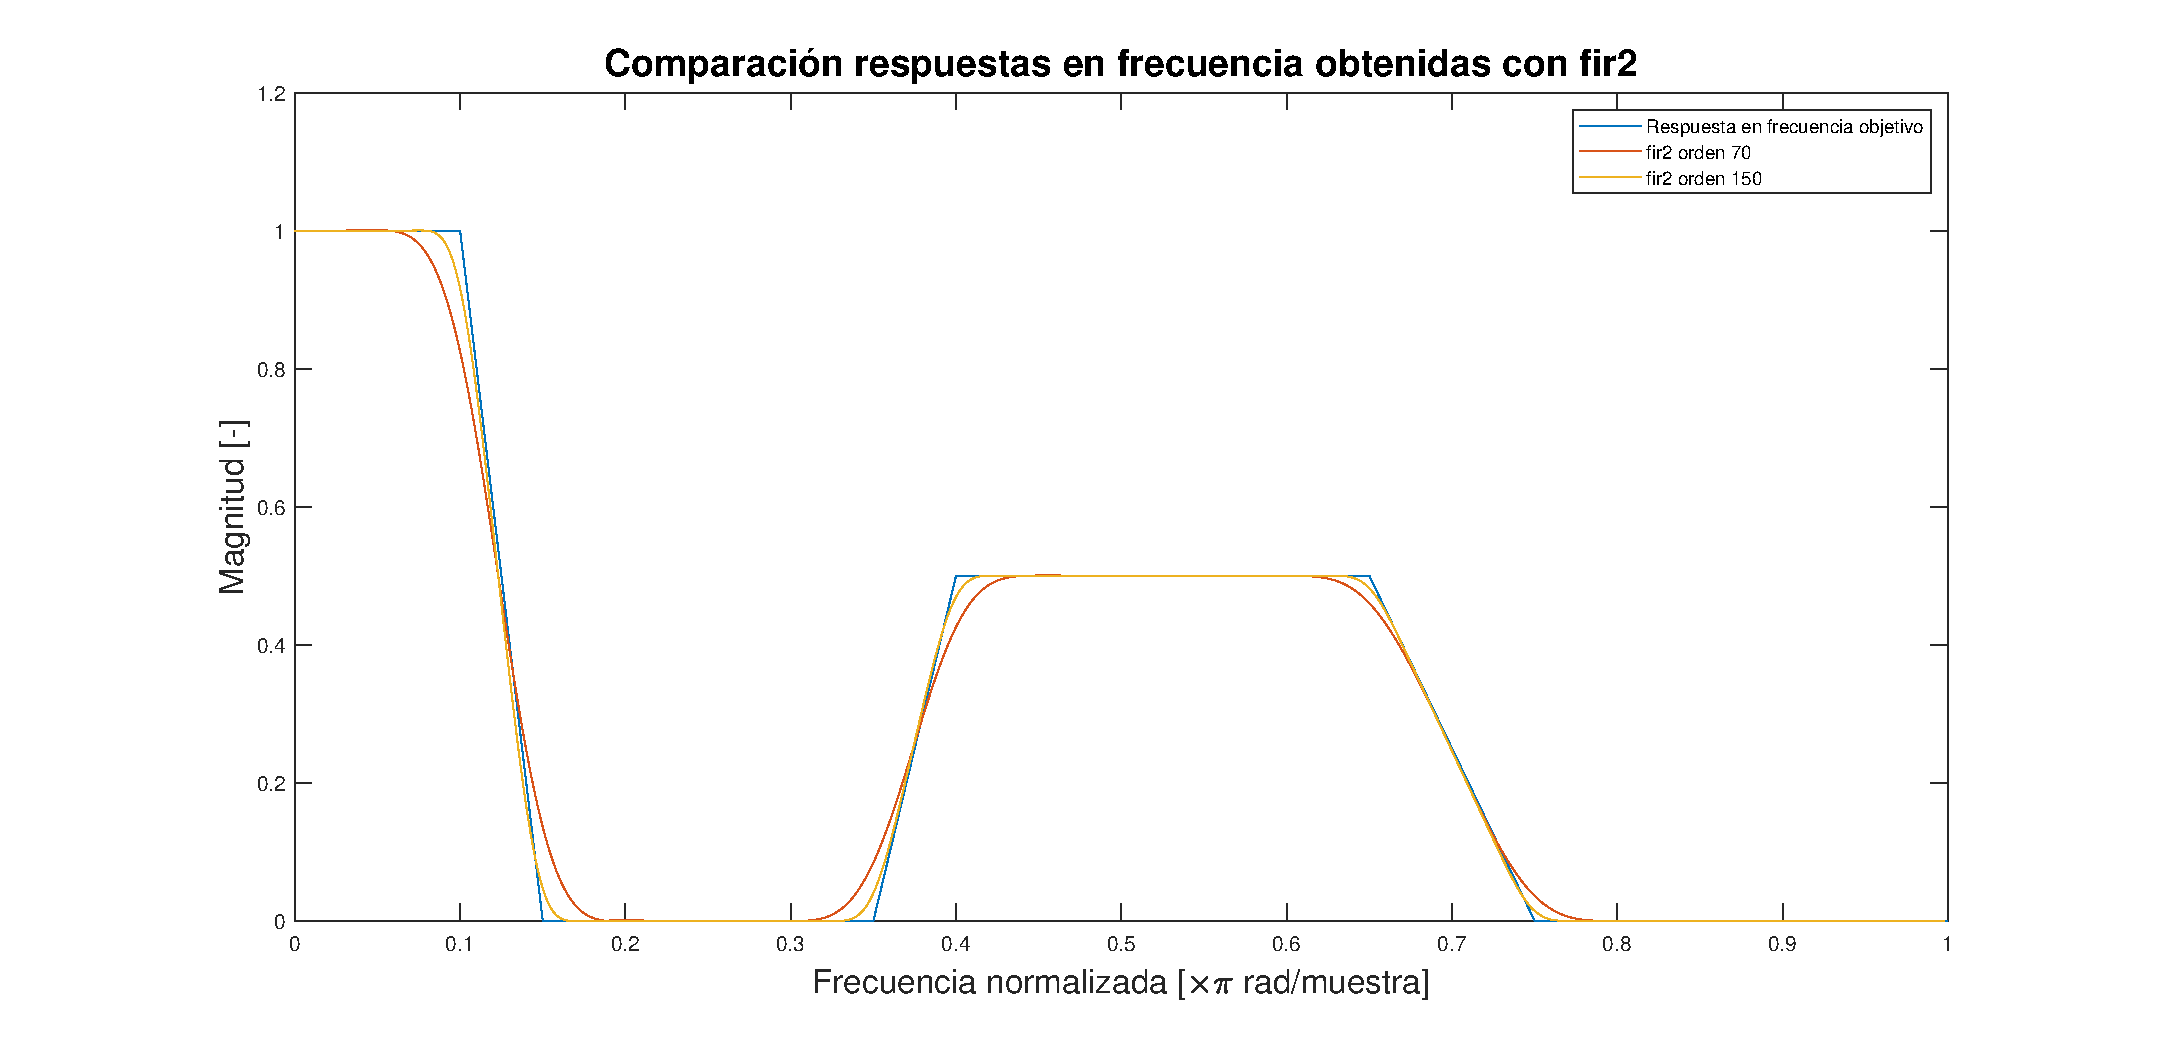
\includegraphics[width = .8 \linewidth]{Figuras/p1_32_FR1.eps}
    \caption{Magnitud de la respuesta en frecuencia de filtro ideal y de diseñados con \texttt{fir2}.}
    \label{fig:p3_2_fr1}
\end{figure}
Posteriormente, para una mejor comparación entre la respuesta en frecuencia de ambos filtros diseñados, se grafica la magnitud de la respuesta en frecuencia en dB, lo cual se muestra en la figura \ref{fig:p3_2_fr2}. 

Se aprecia que no hay gran diferencia en atenuación entre ambos filtros, siendo obviamente el filtro de mayor orden de atenuación más fuerte. La mayor diferencia se aprecia en la banda de transición, la cual es claramente mas abrupta en el filtro de mayor orden. Dependiendo la aplicación esa podría ser una ventaja a considerar.
\begin{figure}[H]
    \centering
    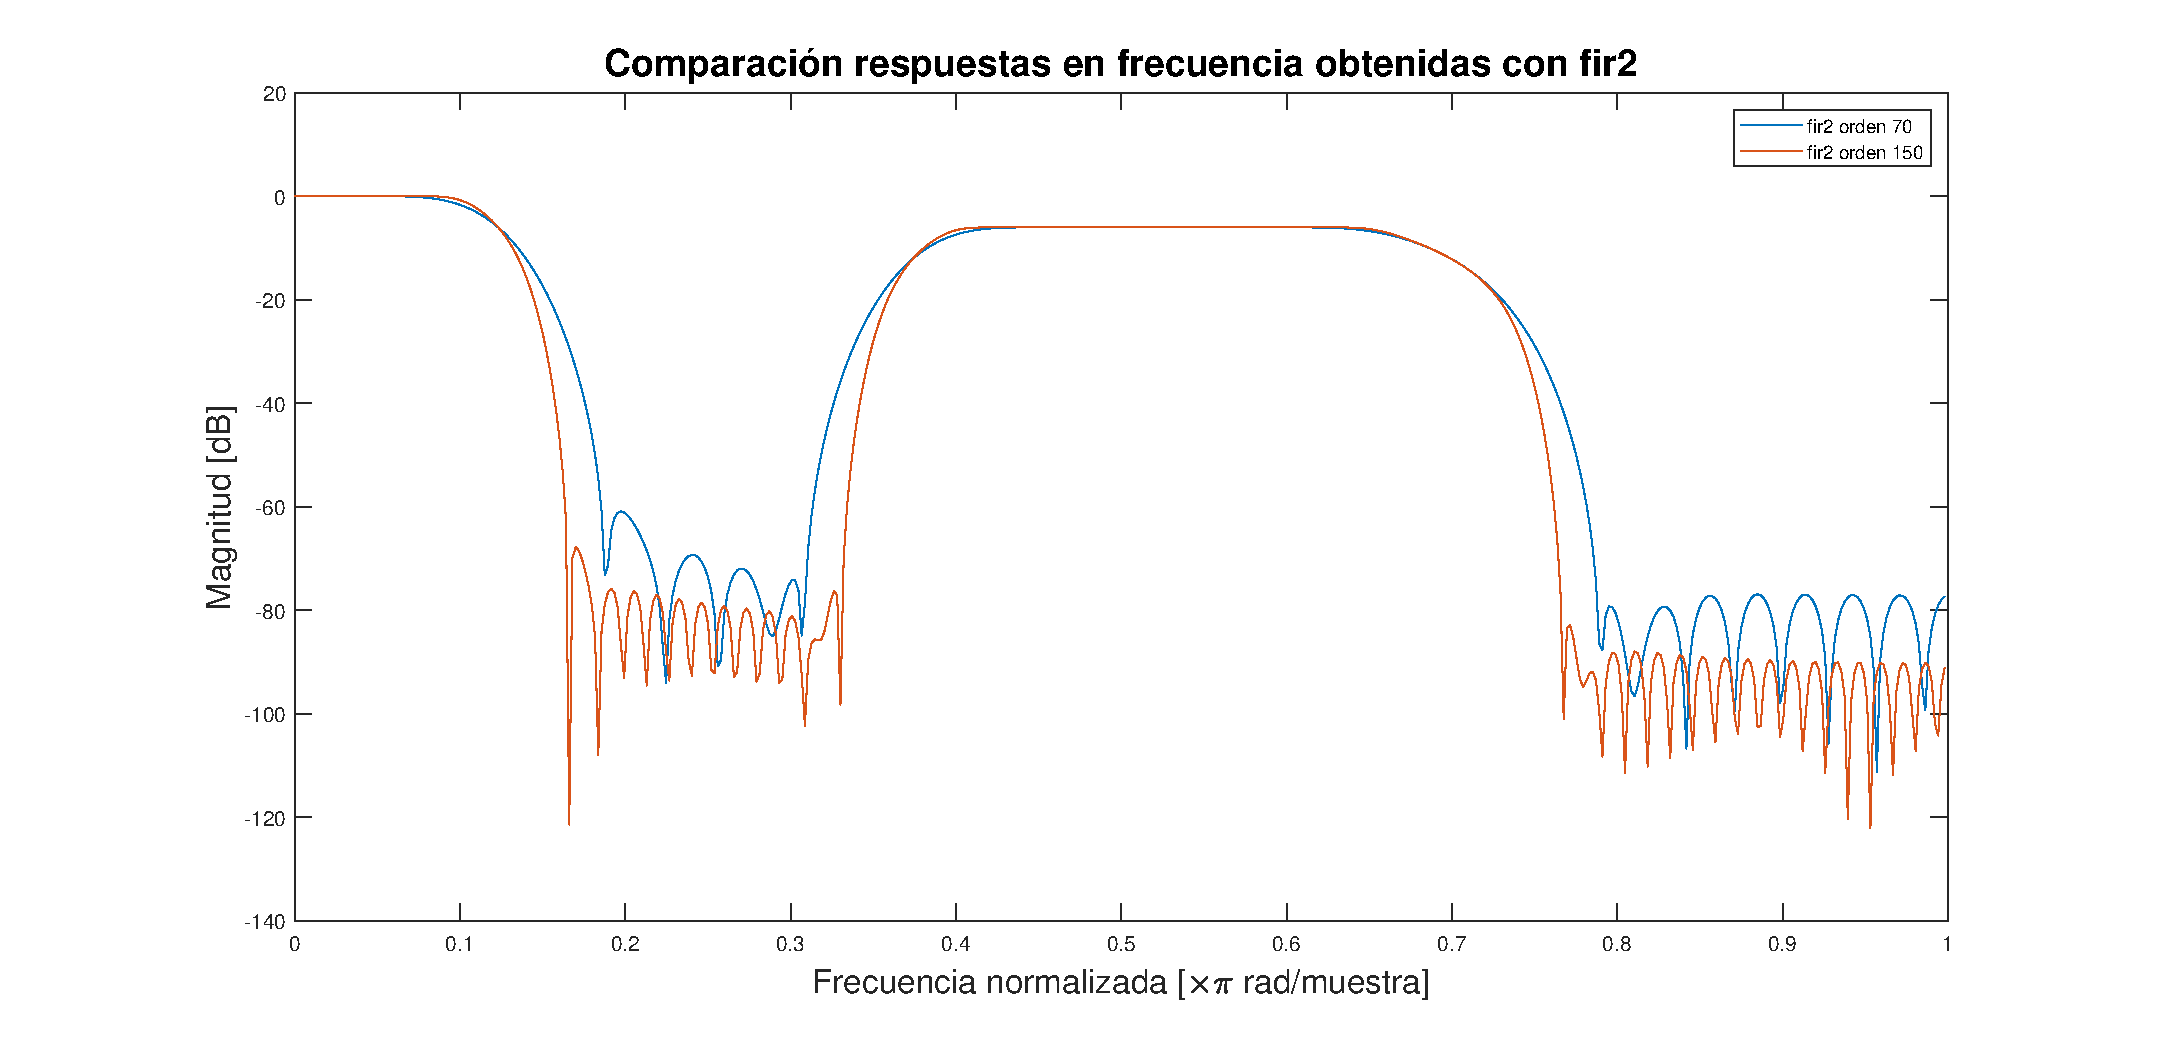
\includegraphics[width = .8 \linewidth]{Figuras/p1_32_FR2.eps}
    \caption{Magnitud de la respuesta en frecuencia de filtro ideal y de diseñados con \texttt{fir2} en dB.}
    \label{fig:p3_2_fr2}
\end{figure}
\item El comando \texttt{firpm} hace referencia al diseño de filtro FIR ocupando el algoritmo Parks-McClellan.

Dicho algoritmo corresponde a un método iterativo para el diseño óptimo de filtros FIR dada una respuesta en frecuencia deseada y sujeto a un orden. Cabe destacar que el criterio de  optimalidad es en el sentido de la norma $\infty$ del error en frecuencia o, en otras palabras, del máximo error absoluto entre la respuesta en frecuencia deseada y la respuesta frecuencia obtenida situando los ceros del filtro.

La sintaxis típica del comando es \texttt{b = firpm(n,f,a)} donde:
\begin{itemize}
    \item \texttt{b}: Vector de coeficientes MA del filtro FIR.
    \item \texttt{n}: Orden del filtro a diseñar.
    \item \texttt{f}: Vector de frecuencias.
    \item \texttt{a}: Vector de amplitudes de la respuesta en frecuencia correspondientes al vector de frecuencias.
\end{itemize}

Una forma de utilizar este comando es en el diseño de filtros chebyshev cuando existe una restricción de ripple para obtener un filtro de bajo orden.

Para lo anterior en primer lugar se ocuparía el comando \texttt{firmord} para estimar el orden del filtro óptimo dada una respuesta en frecuencia deseada junto a sus restricciones de ripple y luego ocupar esa misma respuesta en frecuencia deseada junto con el orden obtenido para la obtención de los coeficientes de \texttt{b} usando \texttt{firpm}.


%\texttt{firpm}: Diseño de filtro FIR óptimo dado una respuesta en frecuencia deseada usando el algoritmo Parks-McClellan. En secciones posteriores se analizará más en detalle.
%Parks-McClellan optimal FIR filter design
%firpm designs a linear-phase FIR filter using the Parks-McClellan algorithm [2]. The Parks-McClellan algorithm uses the Remez exchange algorithm and Chebyshev approximation theory to design filters with an optimal fit between the desired and actual frequency responses. The filters are optimal in the sense that the maximum error between the desired frequency response and the actual frequency response is minimized.
\end{enumerate}